\documentclass{gescons}

\genre {Resumo do Biênio}
\author{Ana Claudia Prado e Magda Stapf Amancio}
\authorrole{Coordenadoras Gerais da Editares}
\title{Da Ideia do Autor às Mãos do Leitor: o Fluxo Editorial Conscienciológico}

\begin{document}
    \makeentrevistatitle
    %\maketitle

    %\fullwidthimage{fields}{b}

    %\coverart{back/editorial}
    \coverart{../fundo-generico.png}
    
%    \begin{multicols}{2}

%\begin{center}
%    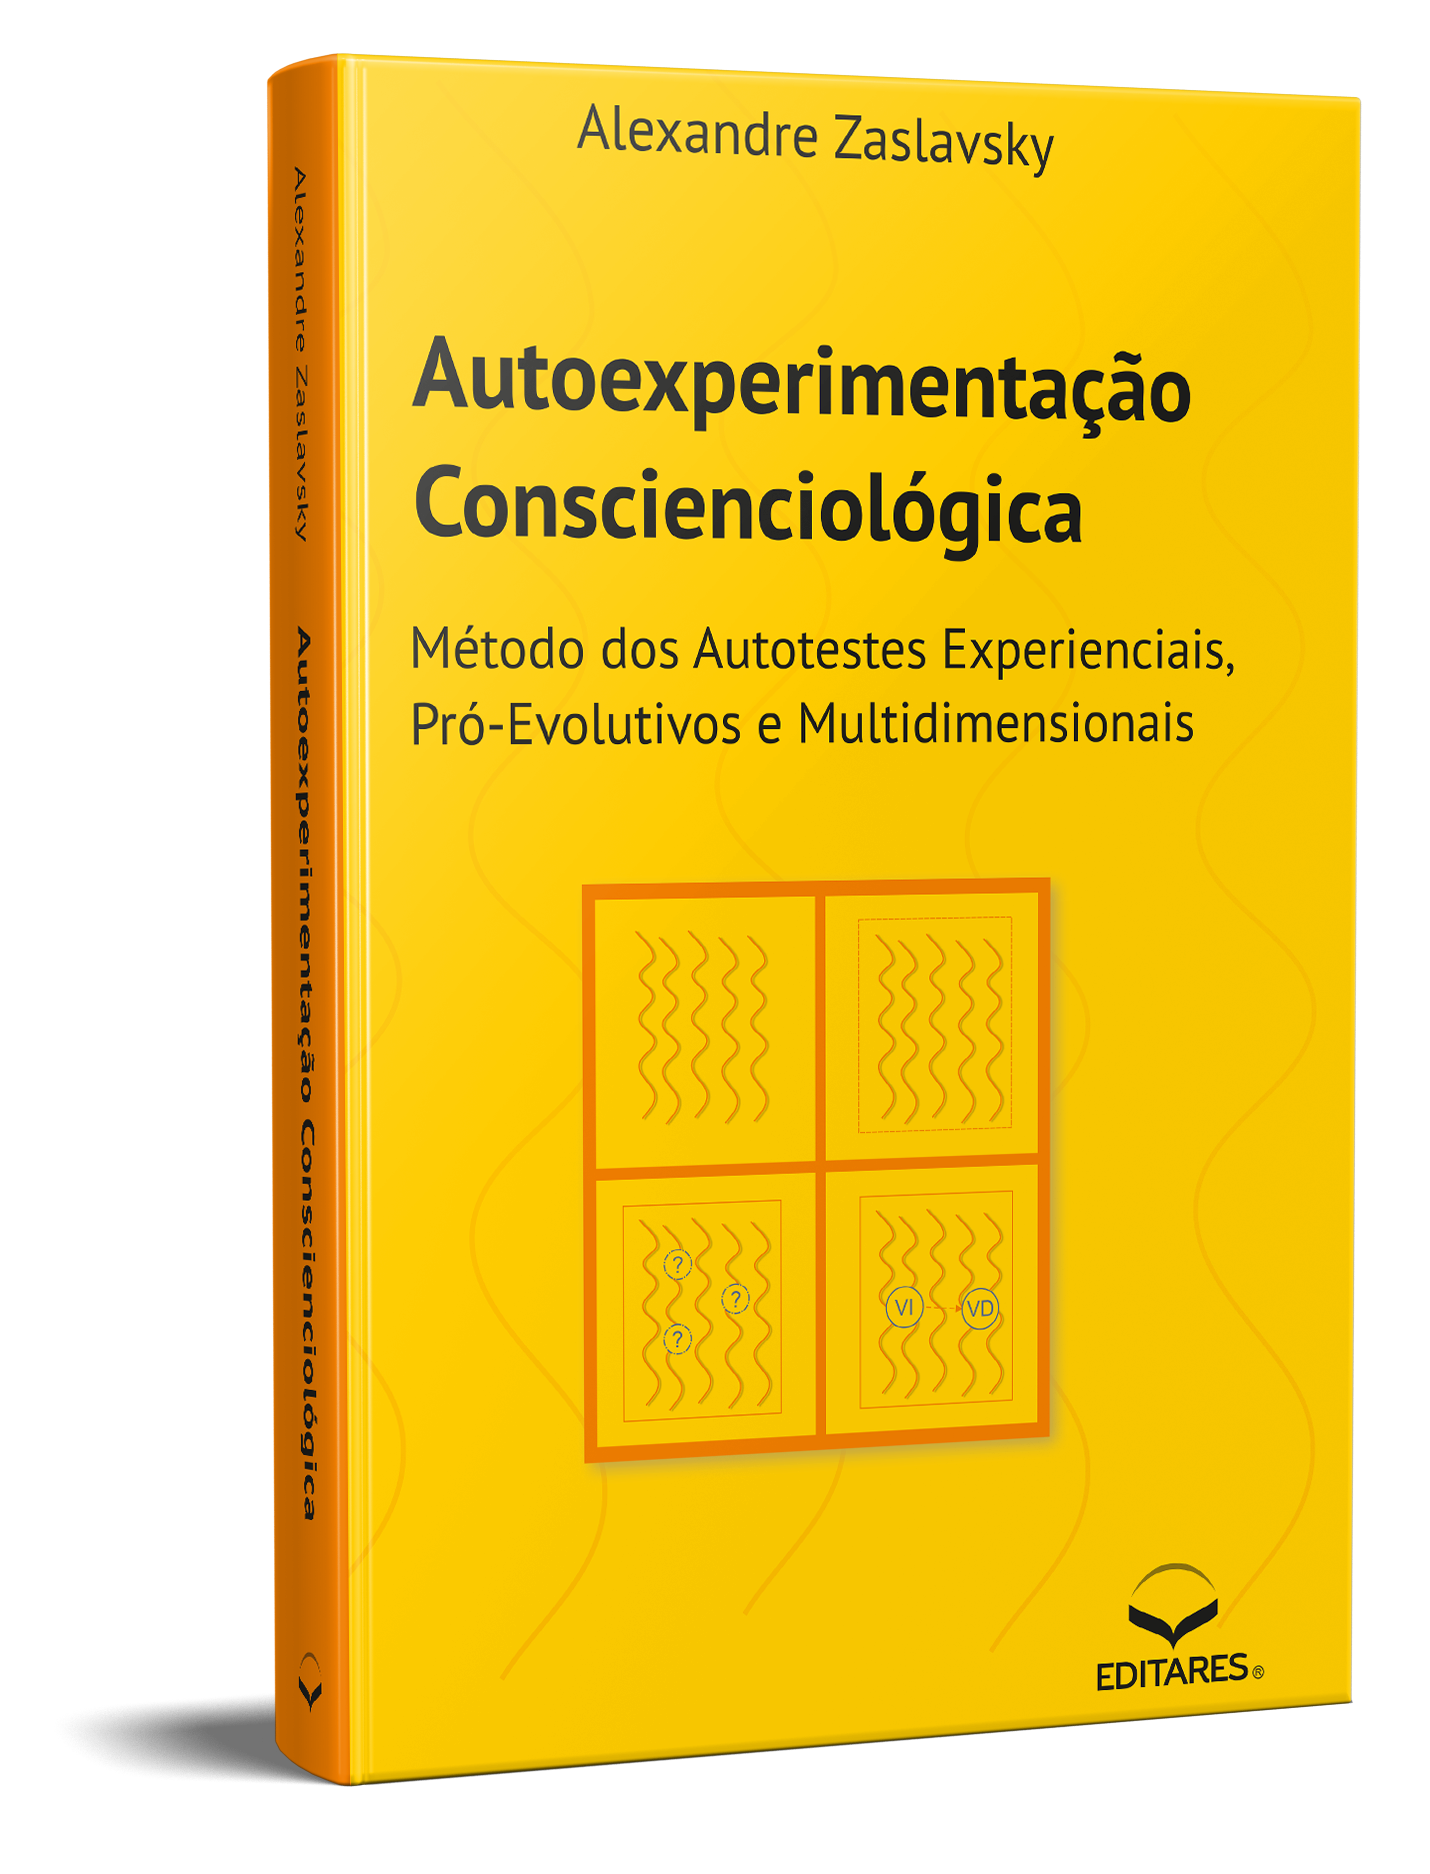
\includegraphics[width=4cm]{articles/entrevista/mockups/Alexandre-Zas.png}
%\end{center}

Publicar um livro não é apenas escrever. Na Editares, cada obra passa por um processo integrado que alia rigor editorial, trabalho voluntário e compromisso interassistencial tarístico para \textbf{garantir qualidade e relevância} antes de chegar ao leitor.

O fluxo editorial começa com o envio dos originais textuais pelo autor para o e-mail da Editares. Em seguida, o material é organizado na plataforma \emph{Trello Editorial} e submetido à pré-análise por uma equipe voluntária, que analisa conteúdo, estrutura e a forma. Quando necessário, o texto retorna ao autor para melhorias até estar pronto para avançar.

Com a aprovação da pré-análise, o material textual ingressa no fluxo formal de produção editorial que contempla parecer técnico, assinatura do termo de cessão de direitos autorais e revisões linguístico-textual e de conteúdo e forma --- conhecidas como \emph{Confor.} Durante esta etapa, o editor e revisores especializados trabalham em parceria com o autor, garantindo autenticidade e qualidade técnica.

Com o texto finalizado, o livro passa para a diagramação, momento em que o conteúdo ganha forma gráfica, tornando-se fluido e agradável à leitura. O autor pode optar pela diagramação voluntária da Editares ou contratar um profissional externo. Antes de seguir para a impressão, uma prova física é cuidadosamente revisada para assegurar o acabamento.

Após a definição do orçamento e da tiragem, a obra é encaminhada para a gráfica. Paralelamente, a equipe de comunicação prepara o lançamento do livro, um \textbf{momento de celebração da conquista do autor} e de início da circulação da obra entre leitores em geral.

Mais do que um produto editorial, cada título publicado pela Editares representa a \textbf{difusão da Conscienciologia,} fortalecendo a interassistência e promovendo o crescimento evolutivo de todos os envolvidos.

% \textbf{FLUXO EDITORIAL DE OBRA CONSCIENCIOLÓGICA}

%\emph{{[}IMAGEM DO FLUXO EDITORIAL ESTÁ NA PASTA FLUXO EDITORIAL{]}}

% \begin{center}
%     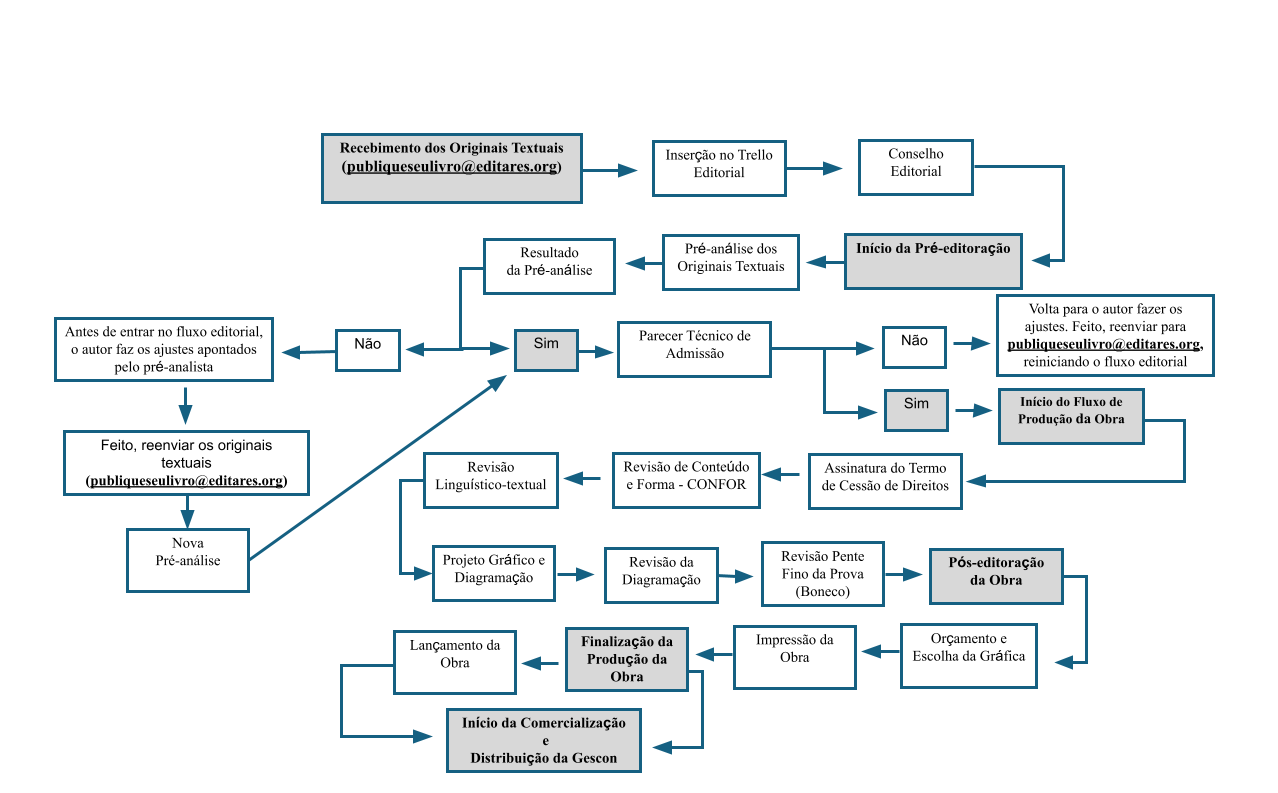
\includegraphics[width=16cm]{articles/resumo/fotos/fluxo-editorial/fluxo-editorial-artigo.png}
% \end{center}

\begin{figure}[h]
  \centering
  \caption*{Fluxo editorial de obra conscienciológica.} % sem numeração
  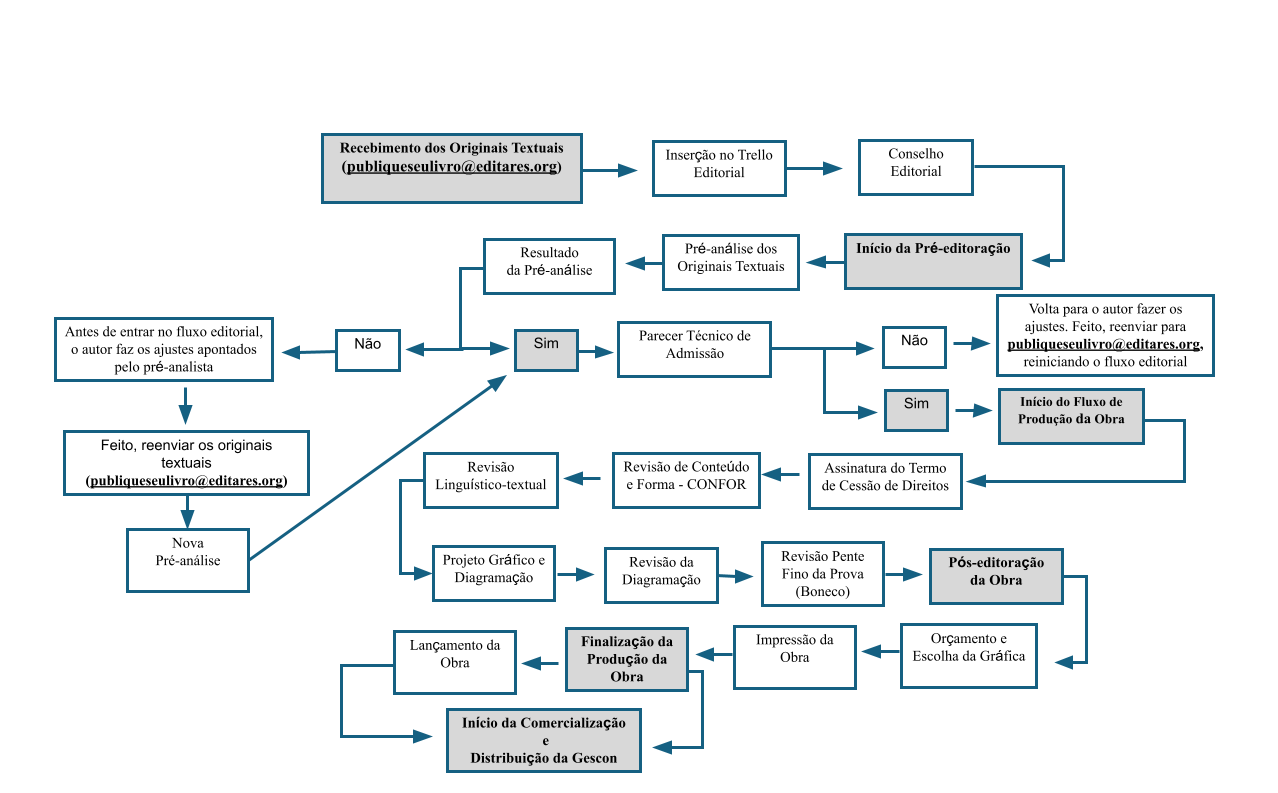
\includegraphics[width=18cm]{articles/resumo/fotos/fluxo-editorial/fluxo-editorial-artigo.png}
\end{figure}


%\noindent
\includegraphics[width=9cm, height=9cm]{articles/resumo/fotos/materia1/IMG20241023143149.jpg}
        
%    \end{multicols}
\end{document}
